% -----------------------------------------------
% Template for ISMIR 2014
% (based on earlier ISMIR templates)
% -----------------------------------------------

\documentclass{article}
\usepackage{ismir2014,amsmath,cite}
\usepackage{graphicx}
\usepackage{amsfonts}
\usepackage{amsmath}
\usepackage{caption}
\usepackage{subcaption}

% Title.
% ------
\title{Analysis of Music Segmentation Boundaries:\\ Machines vs Humans}

% Single address
% To use with only one author or several with the same address
% ---------------
%\oneauthor
% {Names should be omitted for double-blind reviewing}
% {Affiliations should be omitted for double-blind reviewing}

% Two addresses
% --------------
%\twoauthors
  %{First author} {School \\ Department}
  %{Second author} {Company \\ Address}

% Three addresses
% --------------
\threeauthors
  {First author} {Affiliation1 \\ {\tt author1@ismir.edu}}
  {Second author} {\bf Retain these fake authors in\\\bf submission to preserve the formatting}
  {Third author} {Affiliation3 \\ {\tt author3@ismir.edu}}

% Four addresses
% --------------
%\fourauthors
%  {First author} {Affiliation1 \\ {\tt author1@ismir.edu}}
%  {Second author}{Affiliation2 \\ {\tt author2@ismir.edu}}
%  {Third author} {Affiliation3 \\ {\tt author3@ismir.edu}}
%  {Fourth author} {Affiliation4 \\ {\tt author4@ismir.edu}}

\begin{document}
%
\maketitle
%
\begin{abstract}
  The automatic identification of segment boundaries in music has had a strong relevance in the field of Music Information Retrieval in the recent years.
  This task presents many challenges, and arguably the most notable one is the subjectivity of the task itself: two humans do not always agree on the same set of boundaries.
  In this work we present an analysis of this task from two different points of view: machines and humans.
  Five algorithms were selected to segment a dataset of more than 2000 tracks.
  Then we collected multiple human annotations for the 45 hardest tracks and the 5 easiest tracks from a machine point of view.
  The results show that humans' mutual agreement is much higher than machines'.
  We explore the hardest tracks from a machine point of view and the easiest tracks from a human point of view in order to identify the set of audio properties that could potentially improve the current boundary identification algorithms.
  %We present a comparison that aims to shed light into the shortcomings of the current evaluation metrics and discuss a list of properties in the audio that make this task particularly difficult from a machine point of view while humans can 
  
\end{abstract}
%
\section{Introduction}\label{sec:introduction}

Music segmentation intro: focusing on boundaries.

Subjectivity of the task.

Analysis of how machines do vs humans. Aim to improve automatic algorithms.

Organization of the paper.

\section{Boundaries Evaluation Metrics}

The boundaries of a given track are usually evaluated using the hit rate metric.
In this section we review the hit rate, discuss its shortcomings, and explore other metrics that might help addressing our project.
We refer the human annotated boundaries as \emph{reference}, and the ones identified by an algorithm as \emph{estimated}.

\subsection{Hit Rate}

The hit rate for boundaries evaluation is the most common and established metric for this task and it is traditionally used with a specific time window of 3 and/or 0.5 seconds\cite{Ong2005}. 

This metric considers an estimated boundary as \emph{correct} (a hit) if it falls under the specified time window centered at its corresponding reference boundary.
These hits are then used to compute three scores: the Precision (number of hits over the number of estimated boundaries), the Recall (number of hits over the number of reference boundaries), and the F-measure (harmonic mean between Precision and Recall), which is computed as follows:

\begin{equation}
  F = 2 \frac{P R}{P + R}
\end{equation}

\subsection{Median Deviations}

This metric involves the computation of two median deviations: \emph{median reference to estimation} is the median in seconds from the reference boundaries to their nearest estimated ones, and the \emph{median estimation to reference} is analogous but swapping reference boundaries by estimated ones\cite{Pampalk}.
Median deviations are not commonly reported in publications of boundary algorithms since the hit rate tends to be more reliable (note that these median deviations are not normalized and not compacted in a single score like the F-measure).
However, they are, along with the hit rate, the only metrics included in MIREX to evaluate the estimated boundaries.

\subsection{Information Gain}

One of the most reliable metrics for beat tracking is the information gain\cite{Davies2009}. 
This score has successfully been used to identify hard tracks (in terms of beat tracking) from a machine point of view from a large dataset without reference annotations\cite{Holzapfel2012}.
This motivates us to explore its behavior when used for the task of boundary identification.

The idea behind this metric is to treat the error between the reference and the estimation as a probability distribution.
Typically, an error histogram of $K$ bins is used to capture these errors within a certain time range.
The information gain $D$ can be seen as the inverse of the entropy of the probability distribution defined by the error histogram $p(z)$. Formally:

\begin{equation}
  D = \log_2(K) - H(p(z))
\end{equation}

If $p(z_k)$ is the probability mass of the bin $k$ of the error histogram, then $H(\cdot)$, which is the entropy function, can be defined as follows:

\begin{equation}
  H(p(z)) = \sum_{k=1}^K p(z_k) \log_2 \left( \frac{1}{p(z_k)} \right)
\end{equation}

Therefore we obtain a high $D$ if the error distribution is a prominent peak in the histogram (i.e. the error does not vary), whereas $D$ is low, close to 0, if the histogram is uniform (i.e. the error has a high degree of variation and the entropy is high).
$D$ is bounded between 0 and $\log_2(K)$.

Typically, in the task of beat tracking, histograms of $K=41$ bins are used within the range of $\pm0.5$ seconds.
In our case, we use $K=250$ and an unrestricted time range in order to capture the higher errors that manifest in the boundary identification task compared to beat tracking.

\subsection{Trimming First and Last Boundaries}

The presented metrics treat all the boundaries of a given track equally. 
However, we can argue that the first and last boundaries are trivial to be retrieved (the first boundary should always be placed in second 0, and the last one in the second defined by the duration of the track). 
This topic was discussed in the music segmentation breaking sessions of last ISMIR edition\cite{Nieto2013}, and in this work we present two versions of each given evaluation: trimmed and not trimmed.

\section{Machines Identifying Boundaries}\label{sec:eval_desc}

Different approaches: novelty, homogeneity, repetition.

Choosing the five algorithms: OLDA\cite{McFee2014}, Serr\`a\cite{Serra2013},
Foote\cite{Foote1999}, Levy\cite{Levy2008}, SI-PLCA\cite{Weiss2011}.

Talk about the Mean Mutual Agreement and Mean Performance Ground-truth\cite{Holzapfel2012}.

\subsection{Music Segmentation Framework}

Open source project\footnote{Not displayed for revision process.}

Machines.

\subsection{Dataset}

Isophonics, SALAMI\cite{Smith2011}, Cerulean, Ephiphyte.

\subsection{Metrics Comparison}

\begin{figure}
      \centering
      \begin{subfigure}[b]{0.25\textwidth}
              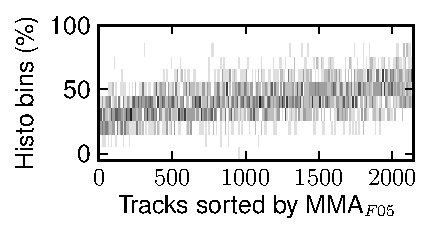
\includegraphics[width=\textwidth]{plots/histo-F05.pdf}
              %\caption{Histogram of F-measure 0.5}
              \caption{}
              \label{fig:histo-F05}
      \end{subfigure}%
      ~ 
      \begin{subfigure}[b]{0.25\textwidth}
              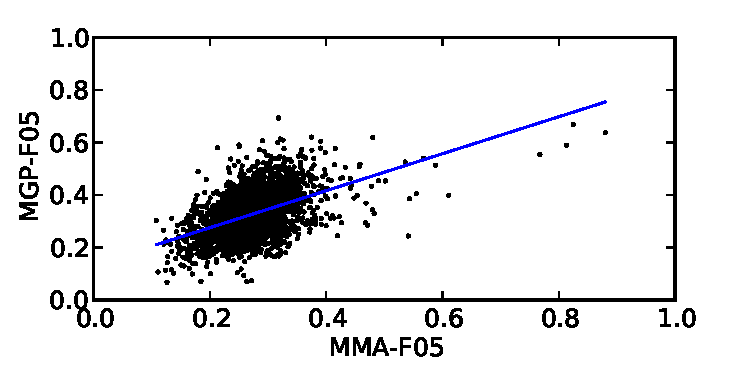
\includegraphics[width=\textwidth]{plots/correl-F05.pdf}
              \caption{}
              \label{fig:correl-F05}
      \end{subfigure}

      \begin{subfigure}[b]{0.25\textwidth}
              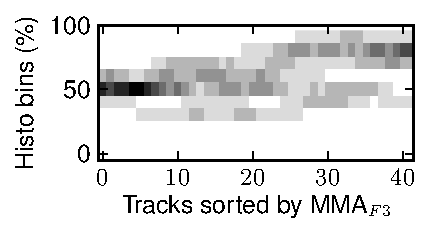
\includegraphics[width=\textwidth]{plots/histo-F3.pdf}
              \caption{}
              \label{fig:histo-F3}
      \end{subfigure}%
      ~ 
      \begin{subfigure}[b]{0.25\textwidth}
              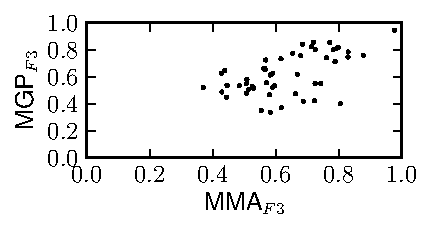
\includegraphics[width=\textwidth]{plots/correl-F3.pdf}
              \caption{}
              \label{fig:correl-F3}
      \end{subfigure}

      \begin{subfigure}[b]{0.25\textwidth}
              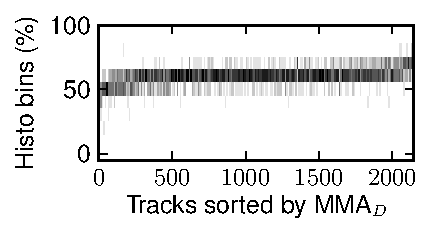
\includegraphics[width=\textwidth]{plots/histo-D.pdf}
              \caption{}
              \label{fig:histo-D}
      \end{subfigure}%
      ~ 
      \begin{subfigure}[b]{0.25\textwidth}
              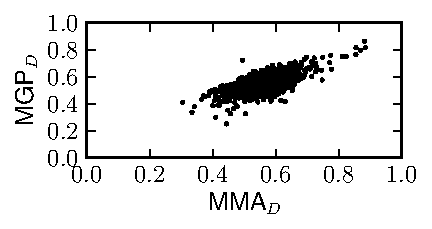
\includegraphics[width=\textwidth]{plots/correl-D.pdf}
              \caption{}
              \label{fig:correl-D}
      \end{subfigure}

      \begin{subfigure}[b]{0.25\textwidth}
              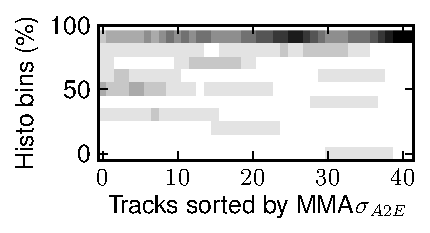
\includegraphics[width=\textwidth]{plots/histo-DevA2E.pdf}
              \caption{}
              \label{fig:histo-DevA2E}
      \end{subfigure}%
      ~ 
      \begin{subfigure}[b]{0.25\textwidth}
              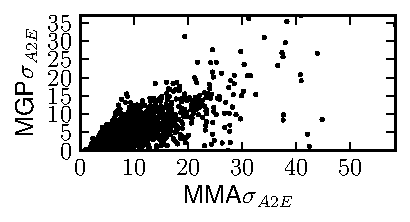
\includegraphics[width=\textwidth]{plots/correl-DevA2E.pdf}
              \caption{}
              \label{fig:correl-DevA2E}
      \end{subfigure}

      \begin{subfigure}[b]{0.25\textwidth}
              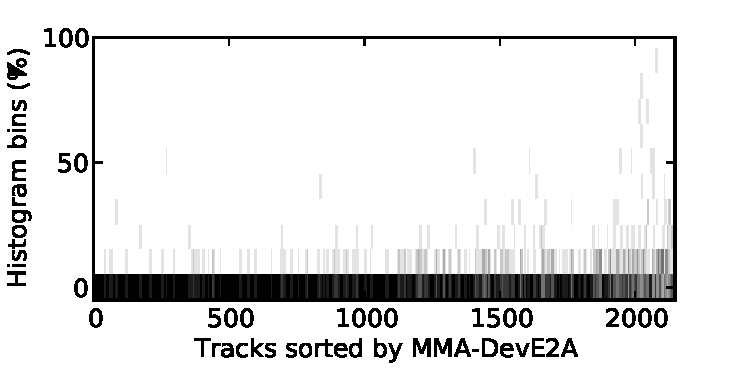
\includegraphics[width=\textwidth]{plots/histo-DevE2A.pdf}
              \caption{}
              \label{fig:histo-DevE2A}
      \end{subfigure}%
      ~ 
      \begin{subfigure}[b]{0.25\textwidth}
              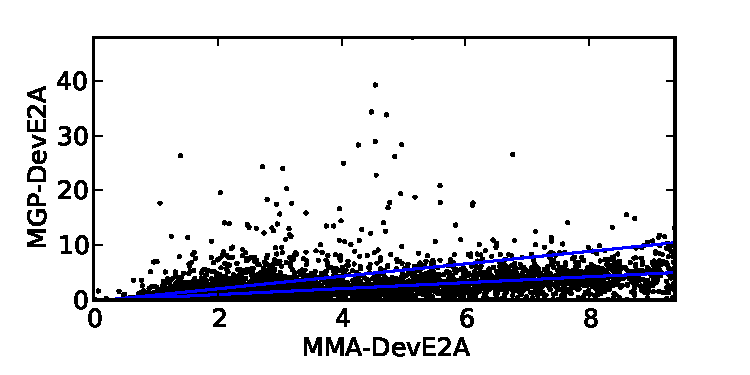
\includegraphics[width=\textwidth]{plots/correl-DevE2A.pdf}
              \caption{}
              \label{fig:correl-DevE2A}
      \end{subfigure}

      \caption{Pictures of animals}\label{fig:animals}
\end{figure}

\subsection{Selection of Hardest and Easiest Tracks}

Plots of MGP and MMA.

\section{Humans Identifying Boundaries}\label{sec:using_method}

Experiment. 5 subjects. 50 tracks: 45 hard, 5 easy.

\subsection{Experiment Setup}

Talk about the SALAMI guidelines.

\section{Machines vs Humans}

Plot comparing MGP-machines vs MGP-humans.

Analyze the answers, display most common problems in a table.

%\begin{table}
 %\begin{center}
 %\begin{tabular}{|l|l|}
  %\hline
  %String value & Numeric value \\
  %\hline
  %Hello ISMIR  & 2014 \\
  %\hline
 %\end{tabular}
%\end{center}
 %\caption{Table captions should be placed below the table.}
 %\label{tab:example}
%\end{table}

%\begin{figure}
 %\centerline{\framebox{
 %\includegraphics[width=\columnwidth]{figure.png}}}
 %\caption{Figure captions should be placed below the figure.}
 %\label{fig:example}
%\end{figure}

\section{Conclusions}

Identified some audio properties that could improve the automatic segmentation algorithms.


%\begin{thebibliography}{citations}

%\bibitem {Author:00}
%E. Author:
%``The Title of the Conference Paper,''
%{\it Proceedings of the International Symposium
%on Music Information Retrieval}, pp.~000--111, 2000.

%\bibitem{Someone:10}
%A. Someone, B. Someone, and C. Someone:
%``The Title of the Journal Paper,''
%{\it Journal of New Music Research},
%Vol.~A, No.~B, pp.~111--222, 2010.

%\bibitem{Someone:04} X. Someone and Y. Someone: {\it Title of the Book},
    %Editorial Acme, Porto, 2012.

%\end{thebibliography}

\bibliography{references}

\end{document}
